%%%%%%%%%%%%%%%%%%%%%%%%%%%%%%%%%%%%%%%%%
% University/School Laboratory Report
% LaTeX Template
% Version 3.1 (25/3/14)
%
% This template has been downloaded from:
% http://www.LaTeXTemplates.com
%
% Original author:
% Linux and Unix Users Group at Virginia Tech Wiki 
% (https://vtluug.org/wiki/Example_LaTeX_chem_lab_report)
%
% License:
% CC BY-NC-SA 3.0 (http://creativecommons.org/licenses/by-nc-sa/3.0/)
%
%%%%%%%%%%%%%%%%%%%%%%%%%%%%%%%%%%%%%%%%%

%----------------------------------------------------------------------------------------
%	PACKAGES AND DOCUMENT CONFIGURATIONS
%----------------------------------------------------------------------------------------

\documentclass{article}

\usepackage[version=3]{mhchem} % Package for chemical equation typesetting
\usepackage{siunitx} % Provides the \SI{}{} and \si{} command for typesetting SI units
\usepackage{graphicx} % Required for the inclusion of images
\usepackage{natbib} % Required to change bibliography style to APA
\usepackage{amsmath} % Required for some math elements 
\usepackage{hyperref}
\usepackage[a4paper,margin=0.5in]{geometry}
\setlength\parindent{0pt} % Removes all indentation from paragraphs

\renewcommand{\labelenumi}{\alph{enumi}.} % Make numbering in the enumerate environment by letter rather than number (e.g. section 6)

%\usepackage{times} % Uncomment to use the Times New Roman font

%----------------------------------------------------------------------------------------
%	DOCUMENT INFORMATION
%----------------------------------------------------------------------------------------

\title{Gate Detection} % Title

\author{Philipp \textsc{Duernay}} % Author name

\date{\today} % Date for the report

\begin{document}
\maketitle
% If you wish to include an abstract, uncomment the lines below
% \begin{abstract}
% Abstract text
% \end{abstract}

%----------------------------------------------------------------------------------------
%	SECTION 1
%----------------------------------------------------------------------------------------

\section{Recap}
In the last meeting from 23.02.2018 several next steps were defined:
\begin{enumerate}
	\item \textbf{Make training data more similar to real test data (Distortion, Noise ..)}
	\item \textbf{Label real data, start with ~5000 images}
	\item \textbf{Investigate how such high speed performance was implemented.}
	\item \textbf{Finally finish SSD}
	\item \textbf{Look into further steps/alternative methods.}
	\item \textbf{Read on transfer learning between synthetic and real data}
\end{enumerate}

\section{Data}

To make the data more realistic a couple of methods were applied. Examples can be seen \autoref{fig:aug}

\begin{itemize}
	\item \textbf{Distortion} The images taken from the bebop camera were from a wide eye lens which could be one reason that the model didn't detect any gate. To mimick such an effect some training images were randomly distorted. So some of the training data has different ranges of distortion. This should avoid overfitting to straight lines and the detector should be more robust.
	\item \textbf{Noise/Blur} The images from the bebop and also from the videos of the drone races have a worse quality than the images created so far. To mimick this effect the training images were blurred with a Gaussian kernel and some Gaussian noise was added. Additionally some of the images were randomly subsampled.
	\item \textbf{Light Sources} The generated data had quite strong shadows due to the added light sources. These was beyond realism so in the new data the light sources are more uniform.
\end{itemize}

\begin{figure}[h]
	\centering
	
	\begin{minipage}{0.24\textwidth}
		\centering
		\includegraphics[width=\textwidth]{fig/org}
	\end{minipage}
	\begin{minipage}{0.24\textwidth}
		\centering
		\includegraphics[width=\textwidth]{fig/noise}
	\end{minipage}
	\begin{minipage}{0.24\textwidth}
		\centering
		\includegraphics[width=\textwidth]{fig/blur}
	\end{minipage}
	\begin{minipage}{0.24\textwidth}
		\centering
		\includegraphics[width=\textwidth]{fig/distort}
	\end{minipage}
	\caption{Examples for Different Image Augmentation Methods (original, noise, blur, distort)}
	\label{fig:aug}
\end{figure}

\section{SSD}

SSD seems to be finally working. The problem was that in the paper it sounded like they labeled all default boxes as background that have an intersection over union of less than 0.5 with any object. However, in the actual code they only use boxes that are lower than 0.2 while everything between 0.2 and 0.5 is just not labeled at all and not taken into account. After changing this the amount of negative boxes was reduced a lot and the training got much more stable. To this end SSD300 was trained on the Pascal VOC dataset and it gives sensible results although a proper test still needs to be done. SSD300 was also trained on the gate data but did not really work so far. The issue could be some hyperparameters which need to be adapted.

\section{Evaluation}

\subsection{Generated Set}

A new test set was generated to test the models. It consists of 1000 images containing 1-3 gates, 1.33 on average. The image augmentation is not applied on the test images. The results can be seen in \autoref{fig:pr} The methods evaluated can be seen in \autoref{tab:models}
\begin{table}[htbp]
	\centering
	\caption{Evaluated Models on the generated data set. Light conditions refers to the training set. "Soft" is the new set generated with less strong light conditions. "Hard" are the models from the previous report".}
	\begin{tabular}{|l|l|l|l|l|l|}
		\hline
		Name & resolution & train samples & augmentation & light cond. & video link \\ \hline
		tinyyolo & 208x208 & 20k & x & soft  &\\ \hline
		tinyyolo & 416x416 & 20k & x & soft & \url{https://youtu.be/-S7RJEH89DQ}\\ \hline
		tinyyolo & 416x416 & 20k &  & soft & \url{https://youtu.be/M1l_9-J3xDI}\\ \hline
		tinyyolo & 416x416 & 10k &  & soft &\\ \hline
		tinyyolo & 416x416 & 10k &  & hard &\\ \hline
		yolov2 & 416x416 & 20k & x & soft & \url{ https://youtu.be/9-H0CvXHyyk}\\\hline
		yolov2 & 416x416 & 20k &  & soft & \url{https://youtu.be/C9aaO7eSs3E}\\\hline
		yolov2 & 416x416 & 10k &  & soft &\\ \hline
		yolov2 & 416x416 & 10k &  & hard &\\ \hline
	\end{tabular}
	\label{tab:models}
\end{table}

\begin{figure}[h]
	\centering

	\begin{minipage}{0.45\textwidth}
		\centering
		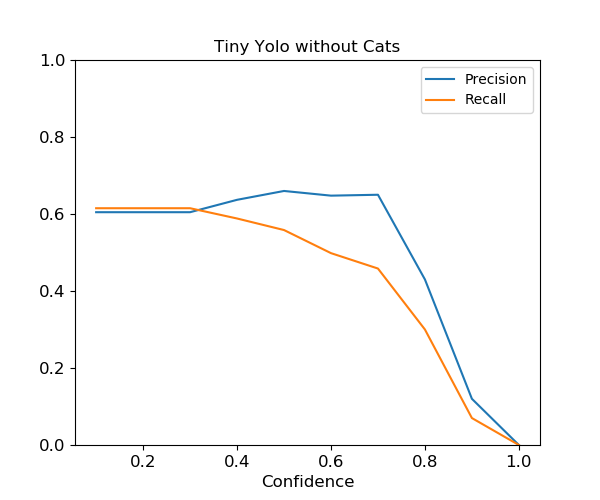
\includegraphics[width=\textwidth]{fig/pr_tiny}
	\end{minipage}
	\begin{minipage}{0.45\textwidth}
		\centering
		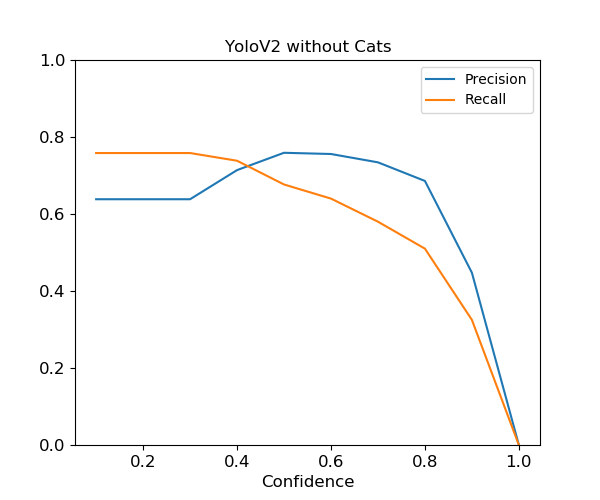
\includegraphics[width=\textwidth]{fig/pr_v2}
	\end{minipage}
	\caption{Average Precision/Recall over generated set.}
	\label{fig:pr}
\end{figure}

On the new data both models get almost comparable results. This is especially surprising as in the first experiments tiny yolo did not work at all. The tiny model with 208x208 resolution and image augmentation gets even comparable results to 416x416 model without augmentation. So it seems that we  don't fully exploit the potential of the far deeper bigger model.

The new models are trained on data that contains the same lightning conditions as the test set. Hence, it makes sense that the new models perform better than the old ones. However, it also means that the old ones overfitted on the strong shadows. 

On the new set we can also see how more samples benefit the prediction. This is different to the results obtained in the last report where the best results could be obtained with 10k train samples.

The image augmentation did not benefit the performance on the test set. However, this makes sense as the test set does not have the distortion/noise conditions as the real data.

In general the methods perform much better than in the last report. One can assume that the new test set is a bit easier as the there are less strong shadows and the color serves as a good feature. Especially the models trained on these light conditions can exploit that fact. Also a higher training size now increased the performance of the models.

\subsubsection{More Detailed}

Among the above listed methods the two best performing are investigated further. \autoref{fig:detail} shows precision recall and number of predictions over confidence levels.
\begin{figure}[h]
	\centering
		
		\begin{minipage}{0.32\textwidth}
			\centering
			\includegraphics[width=\textwidth]{fig/prec_rec_v2}
		\end{minipage}
			\begin{minipage}{0.32\textwidth}
				\centering
				\includegraphics[width=\textwidth]{fig/n_pred}
			\end{minipage}
	\begin{minipage}{0.32\textwidth}
		\centering
		\includegraphics[width=\textwidth]{fig/prec_rec_tiny}
	\end{minipage}
	\caption{Precision/Recall/Number of predictions over confidence. The plots are an average over all test samples. Note that the precision is undefined when there are now predictions. Commonly it is set to zero in that case, which leads to the decrease in precision across the second half.}
	\label{fig:detail}	
	\begin{minipage}{0.45\textwidth}
		\centering
		\includegraphics[width=\textwidth]{fig/hist_v2}
	\end{minipage}
	\begin{minipage}{0.45\textwidth}
		\centering
		\includegraphics[width=\textwidth]{fig/hist_tiny}
	\end{minipage}
	\caption{Histograms for the amount of predictions/true positives at that confidence level. Bin size is 0.1. We see that the confidence mostly reflects the true label. From 0.7 the predictions are correct in most cases.}
	\label{fig:hist}

\end{figure}

\subsection{Real Data}

The interpretability of the results on the generated set are a bit limited as it also depends a lot on how the data is generated. Hence the methods are also evaluated on real data. Namely, two "data sets" exist one is the labeled data by Shuo (MAVLab set). It consists of 500 images taken from the bebop camera. Another set can be taken from the videos of IROS 2017. Some of the images were labeled, however the court contains pretty challenging gates that are even hard to detect for a human. We should agree on how we could best use this as a test set. The performance is still quite poor so no quantitative evaluation has been done, but examples can be seen in the videos as linked in \autoref{tab:models}. Also \autoref{fig:real_tiny} and \autoref{fig:real_tiny_noaug} show some examples.

\begin{figure}[htbp]
	\centering
	
	\begin{minipage}{0.49\textwidth}
		\centering
		\includegraphics[width=\textwidth]{fig/yolov2_noaug_iros_50}
	\end{minipage}
	\begin{minipage}{0.49\textwidth}
		\centering
		\includegraphics[width=\textwidth]{fig/yolov2_iros_54}
	\end{minipage}
	\caption{Example images for the big version of yolo without (left) and with (right) augmentation}
	\label{fig:real_tiny_noaug}
	
	\begin{minipage}{0.49\textwidth}
		\centering
		\includegraphics[width=\textwidth]{fig/tiny56}
	\end{minipage}
	\begin{minipage}{0.49\textwidth}
		\centering
		\includegraphics[width=\textwidth]{fig/tiny125}
	\end{minipage}
	\caption{Example images for the tiny version of yolo on the iros video with image augmentation}
	\label{fig:real_tiny}
\end{figure}

Generally, we see quite poor performance in the first half of the track. However, this also contains the hard gates that were not part of the training data yet. In the second half where the gates are more visible we get some good predictions.

The image augmentation using noisy/blur/distortions does not seem to benefit the performance on the IROS set. Especially the big model produces way more false positives than without using the augmentation \autoref{fig:real_tiny_noaug}(right).

In the video especially we see a lot of false positives on the pole of the gates \autopageref{fig:real_tiny}(left). Probably it detects it as a gate from the side. However, it does not make sense to predict so many, so closely overlapping boxes as this never happens in real/in the training data. Potentially, we can get rid of this by tuning some hyperparameters like anchor box size/non-max suppression but maybe we can also do something smarter.

By visual inspection it seems that false positives often only appear in one frame or are changing a lot in size while confident good predictions stay the same across several frames. Hence, a sequence based approach could potentially increase the performance quite a bit.


\begin{figure}[htbp]
	\centering
	
	\begin{minipage}{0.24\textwidth}
		\centering
		\includegraphics[width=\textwidth]{fig/shuo_v239}
	\end{minipage}
	\begin{minipage}{0.24\textwidth}
		\centering
		\includegraphics[width=\textwidth]{fig/shuo_v261}
	\end{minipage}
	\begin{minipage}{0.24\textwidth}
		\centering
		\includegraphics[width=\textwidth]{fig/shuo_v277}
	\end{minipage}
	\begin{minipage}{0.24\textwidth}
		\centering
		\includegraphics[width=\textwidth]{fig/shuo_v2154}
	\end{minipage}
	\caption{Example images for the big version of yolo on the mavlab set}
	\label{fig:real_yolov2_shuo}
	
	\begin{minipage}{0.24\textwidth}
		\centering
		\includegraphics[width=\textwidth]{fig/shuo_tiny39}
	\end{minipage}
	\begin{minipage}{0.24\textwidth}
		\centering
		\includegraphics[width=\textwidth]{fig/shuo_tiny61}
	\end{minipage}
	\begin{minipage}{0.24\textwidth}
		\centering
		\includegraphics[width=\textwidth]{fig/shuo_tiny77}
	\end{minipage}
	\begin{minipage}{0.24\textwidth}
		\centering
		\includegraphics[width=\textwidth]{fig/shuo_tiny154}
	\end{minipage}
	\caption{Example images for the tiny version of yolo on the mavlab set}
	\label{fig:real_tiny_shuo}
\end{figure}

The results on the MAVLab set are as poor as before. We get some more predictions now but they are really off. This could also be due to the poor quality and resolution of the test images. In a next step we could try to mimick the test data as close as possible to see if that improves the predictions.


\subsection{Speed}

The last measurements were measured in a simple way in python. That way the measured time also contains the communication with tensorflow and maybe even the loading of the computational graph (depends on how keras works internally). To get a better measurement tensorflow supports profiling but that takes some time to configure and will be done in a next step.

\section{Next Steps}
\begin{enumerate}
		\item \textbf{Finish labeling of video to quantify results better}
		\item \textbf{Measure speed with tensorflow profiling}
		\item \textbf{Try to make ssd work on gate data}
		\item \textbf{Investigate sequence based approach}
		\item \textbf{Read on transfer learning between synthetic and real data}
		\item \textbf{Generate training data similar to MAVLab set}
\end{enumerate}


%----------------------------------------------------------------------------------------


%----------------------------------------------------------------------------------------
%	BIBLIOGRAPHY
%----------------------------------------------------------------------------------------

\bibliographystyle{abbrv}

\bibliography{literature}

%----------------------------------------------------------------------------------------


\end{document}\grid
